\documentclass[titlepage]{article}
\usepackage{array}
\usepackage{enumerate}
\usepackage{graphicx}
\usepackage{listings}

\begin{document}

\author{Stevan Stanisic and Santana Mach}
\title{COMP 8505 - Assignment 2 \\ Backdoor}
\date{Oct 19, 2011}
\maketitle{}

\tableofcontents
\pagebreak

\begin{abstract}

In this experiment we pulled together code samples that comprised
a simple Linux backdoor program and implemented some improvements
that would aid in keeping the program from administrators monitoring
the network and machine.

We added DES encryption, process masking and some simple CPU
throttling code so that the backdoor would stand out less. We then
ran a set of utilities that administrators would likely use to try
and find our backdoor, like snort, top, ps, netstat and nmap to
see if it was visible.

What we found was that it would be very difficult to spot the
backdoor even for a reasonably well trained sys-admin. They would
likely have a better chance of detecting the initial intrusion than
the subsequent backdoor activity.

\end{abstract}

\section{Introduction}

The purpose of this experiment is to familiarize ourselves with the
libpcap packet capture library and implement a few improvements to the
backdoor code that has been made available to us. The basic backdoor
program functions as a quiet server (in that it does not respond to at
all to packets not addressed to it). It is, however, not very stealthy
yet for a number of reasons:

\begin{enumerate}
	\item It outputs command results to stdout
	\item It receives commands in plaintext
	\item It makes no attempt to hide its process identifier
	\item It always shows up in top due to excessive CPU usage
\end{enumerate}

Furthermore, a nice to have would be the ability to see the results of
your commands on the compromised machine so that you don't have to guess
whether a command worked or not.

We will attempt to address all these shortcomings with this updated
backdoor program.

\section{Instructions and Usage}

The program is fairly simple to use, both the client and server have
been integrated into the same executable.

The server(backdoor) side only needs to set the ``-s'' flag to denote 
server mode. Optionally, the user can set the ``-d'' flag to send
encrypted results back to the client or add a filter string if they
wish to listen for a different set of packets than ``udp port 53''.

The client(command) side needs to set the ``-c'' flag to denote client
mode and should probably set the ``-i <ip>'' and ``-p <port>'' flags
to specify where to send commands. Optionally, the ``-d'' flag can be
used to listen for and print out command results, but keep in mind that 
the backdoor will reflect responses back on the same port and an
attentive administrator may notice this.

\clearpage

\section{Design}
We will first assume that the person using this program will take the
approprate steps to hide this program on the compromised system. We
will be assuming the executable has the ability to raise its privelege
level to root, but that should automatically
raise flags. A better solution would be to hide it in /sbin and add
it to the startup scripts like any other daemon. We won't concern
ourselves too much with administrative issues like this as they are
outside the scope of our experiment.

\begin{figure}[htb]
  \begin{center}
    \includegraphics[width=0.9\textwidth]{pics/net_diag.png}
  \end{center}
  \caption{Basic Backdoor Setup}
  \label{fig:ntp_packet_image}
\end{figure}

The stealth feature at the core of this backdoor is its ability to
listen passively at such a low level. To an administrator, any command
packets will likely look like they were rejected by the machine if
there is no other service listening on that port (ICMP destination port
unreachable). If the host's firewall is dropping packets to that port,
it will be even less noticeable as there won't be any responses.
Even better, there will be no indication of a listening port if an
administrator runs netstat.

To address the first shortcoming, outputting to stdout (which could
alert a user depending on how the program was started) with our solution
to the last problem, having no way to gather command output. We'll
instead use the popen to launch the command and provide us with a pipe
which we can use to gather output and optionally send back to the 
client.

Now, due to the second shortcoming we have identified, this will look
-extremely- suspicious to an alert network administrator as they will
have what look like shell commands coming in over a known and likely
monitored port (otherwise it's unlikely we could get past the router)
with human readable output going the other way. We will be introducing
DES encryption in both directions so that this is less obvious, but we
cannot encrypt the header key or the backdoor would have to attempt to
decrypt the first few bytes of every packet it received. Our suggestion
here is to modify the key (located in defs.h) to a set of non-printable
characters.

Masking the process id proved to be fairly trivial, we chose to use
the udev daemon as our cover as it runs on nearly all Linux machines,
often in multiple processes, so it will be easy for an admin to
overlook.

Finally, we had to address the CPU usage, because any admin worth their
salt will notice a runaway process like this very quickly. It appears
that pcap\_loop uses busy waiting to process packets, which is less
than ideal so we've decided to use the pcap\_dispatch functionality
instead. It will process a bufferful of packets and then return control
to our program so that we can sleep for a bit and let the buffers fill
back up, bringing our CPU usage down to typical levels for the service
we're emulating.

The basic flow of the Packet Handler function has not changed 
significantly, we have simply added a bit of functionality to it:

\begin{lstlisting}
Packet Handler Function
\{
	...

	since packet has header key, decrypted properly, contains header
	and footer
		execute the system call
	
*	if duplex mode is active
*		send the results back to the client
\}
\end{lstlisting}

\clearpage

The client portion of the program is much simpler to implement as
it can use standard UDP sockets to send and receive data from the
backdoor. The basic command flow should be as follows:

\begin{lstlisting}
Client Function
\{
	initialize outgoing socket

	if duplex mode is active
		initialize incoming socket in separate thread

	loop while until no more user input
		read input
		add header key to outgoing packet
		add protocol header/footer to outgoing packet
		encrypt outgoing packet
		send outgoing packet to backdoor
\}
\end{lstlisting}

As the client is unlikely to be a busy site, it is acceptable to
simply have it attempt to decrypt all incoming packets and attempt
to display them if duplex mode is active. A nicety would be to
add authentication to the results in the same way that commands
are handled, but the fact that we're responding to what should have
been rejected packets in the first place makes this a bit of a moot
point.

\clearpage

\section{Testing}

For the testing, we demostrate that the backdoor works as a backdoor should; undercover
and potentially dangerous.  We split the testing section into the application side and
the detection side.  The application will show that the client can execute the command
on the server end.  The detection section will show or not show the backdoor using
various tools.

\subsection{Application}

The backdoor allows the user to execute commands on the target machine by sending a UDP
packet with a specific signature.  The rest of the payload contains the command with
some checks.  The server will decrypt the rest of the payload and execute the specified
command.\\

\begin{figure}[htb]                                                                       
  \begin{center}
    \includegraphics[width=0.9\textwidth]{pics/serduplex.png}
  \end{center}
  \caption{Backdoor Server in Duplex Mode}
  \label{fig:ser_duplex}
\end{figure}

After the server is executed, it will sit there and listen for commands with the signature
in the payload.  The server will not display any messages as it would not be a reliable
backdoor if it shows the target what is happening.  In duplex mode, the server will reply
with the outputs of the command.\\

\begin{figure}[htb]                                                                       
  \begin{center}
    \includegraphics[width=0.9\textwidth]{pics/cliduplex.png}
  \end{center}
  \caption{Backdoor Client in Duplex Mode}
  \label{fig:cli_duplex}
\end{figure}

Once the target is specified, the user can execute any command as if it is a local machine
(as long as the backdoor is running. In this test, we run the "ls" command to show that
we are in the machine.  Since it is set to duplex mode, we can see the results of the
command.  Local execution of the backdoor will result in the line with the symbols but
will not show during remote execution.\\

\begin{figure}[htb]                                                                       
  \begin{center}
    \includegraphics[width=0.9\textwidth]{pics/tcpdump.png}
  \end{center}
  \caption{tcpdump of Duplex Mode}
  \label{fig:dump_duplex}
\end{figure}

The tcpdump shows or rather, does not show any part of the command in the payload.
The only characters visible in the payload is the header key or signature we use
to authenticate the packet for the backdoor. We use a signature that may also look
like encrypted data to avoid any suspicion.  The signature can be seen in the first
packet as ``(P\^{}.\^{})=P`` .\\

\clearpage

\subsection{Detection}

This section demostrates where the application sits on the target machine.  Using
various tools, we will show if the backdoor is reveal and how we hide it to prevent
detection or suspicion.  The application is masked to look similar to a process that
is common to linux machines.\\

\begin{figure}[htb]                                                                       
  \begin{center}
    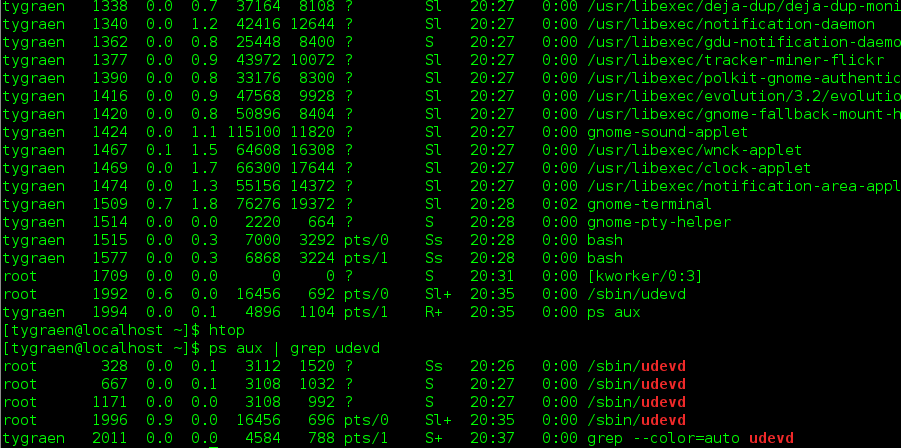
\includegraphics[width=0.9\textwidth]{pics/ps.png}
  \end{center}
  \caption{Backdoor Process}
  \label{fig:bkdoor_ps}
\end{figure}

The ps command shows that the backdoor is running but is masked as\\
''/sbin/udevd -d``. Without circling the backdoor, the process list will not seem
out of the ordinary for the average user.  A more observant user may notice that
the process is quite new or close to the bottom of the process list.  For testing
purposes, we ran the backdoor manually but it should be ran as part of the startup
which will sit nicely between the processes.\\

\begin{figure}[htb]                                                                       
  \begin{center}
    \includegraphics[width=0.9\textwidth]{pics/top.png}
  \end{center}
  \caption{top with Backdoor Server}
  \label{fig:bkdoor_top}
\end{figure}

Similar to the process list, the top command shows the backdoor but under the mask.
The PID is quite high but as said previously, the process should be ran on startup
to hide the application.  The memory usage is relatively low and is stable, therefore it
won't be seen as a suspicious process.\\

\clearpage

\begin{figure}[htb]                                                                       
  \begin{center}
    \includegraphics[width=0.9\textwidth]{pics/nmap.png}
    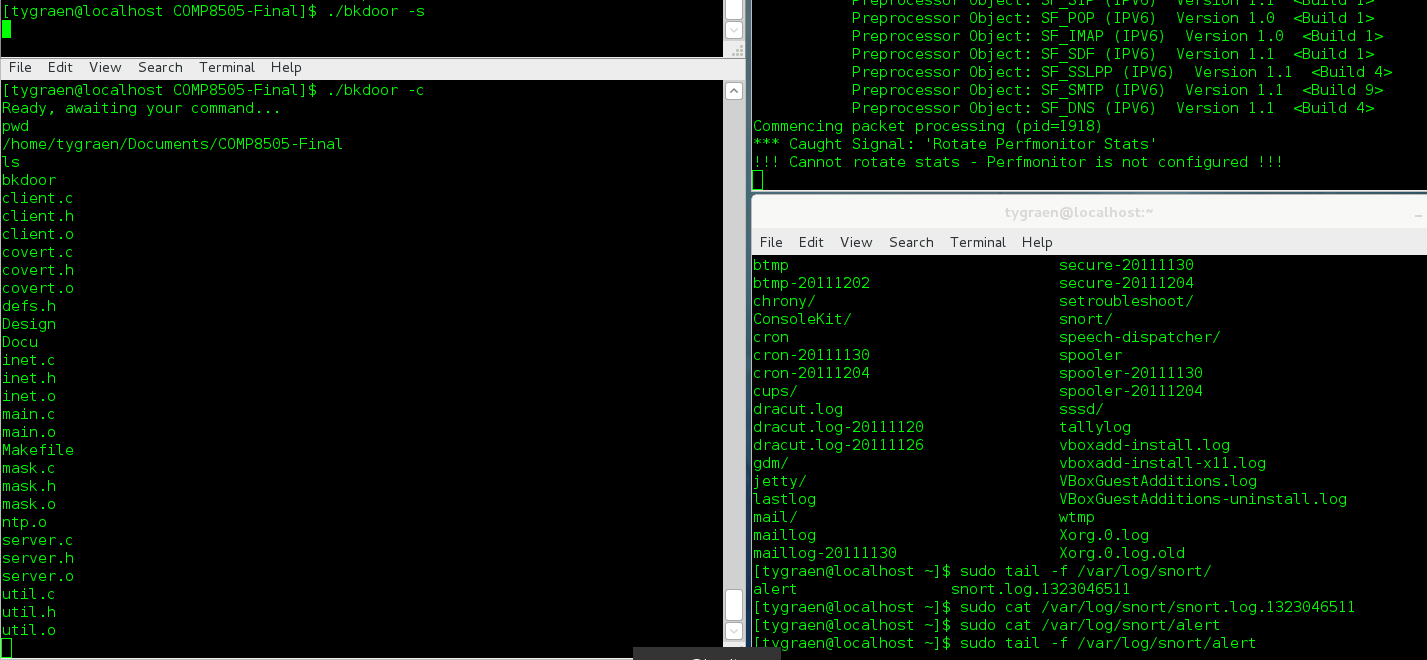
\includegraphics[width=0.9\textwidth]{pics/snort.png}
  \end{center}
  \caption{NMAP and Snort}
  \label{fig:bkdoor_nmap_snort}
\end{figure}

NMAP and Snort both fail to detect that the backdoor is running. The nmap scan shown
does not reveal that port 53 (which the server is listening on) is open.  Similar to
nmap, Snort does not get alerted for sending or executing the command.  This shows
that it is not detectable under normal rulesets on snort.  Even if a rule is made
for the current backdoor, we can change the signature or delay the packets.  The only
possible way is to monitor all machines and keep their history, but that is unreasonable.\\

\clearpage

\section{Conclusion}

For the most part, we accomplished our goals of learning about
how to use the libpcap library and implemented a reasonably
useful backdoor program. In a real world scenario, the client
and server portions of the program should really be separate
executables both to reduce the program's size as well as to
give forensic analysts fewer pieces of the puzzle to work with.
It would be interesting to explore just how small the program
could be if the relevant cryptography and packet capture routines
were pulled directly into the program. As it stands, it compiles
down to only 14KB, but that's still fairly large for the small
amount of functionality that it holds.

We did find it somewhat surprising how easy it is to camouflage
a running process so that even an alert administrator would be
hard pressed to find it without keeping some sort of system
monitoring tool on every host. If the program was compiled
into a commonly used daemon such as apache, it would be near
impossible to detect and solve the problem of having to add an
entry to the startup scripts, however, with that comes the
possibility of an update replacing the backdoor. The logical
extension is to somehow build the code into the bootloader (ie. grub),
however, that is still beyond our reach.

As far as possible network defenses that might be implemented to
detect such behaviour, there isn't any conceivable way to that we
could think of to detect a one-way channel that wouldn't also cause
a large number of false positives any time someone scanned a
computer. It might be possible to write an IDS rule to look for
the result packets coming back in response to the supposedly
rejected packets, but this could be defeated by switching to
another protocol or introducing a delay. In the end, the only real
defense seems to be to not let attackers infiltrate a system in the
first place.

\clearpage

\section{Appendix A}
Snort packet capture statistics:

\begin{lstlisting}
Run time for packet processing was 957.312174 seconds
Snort processed 194 packets.
Snort ran for 0 days 0 hours 15 minutes 57 seconds
   Pkts/min:           12
   Pkts/sec:            0
==================================================
Packet I/O Totals:
   Received:          246
   Analyzed:          194 ( 78.862%)
    Dropped:            0 (  0.000%)
   Filtered:            0 (  0.000%)
Outstanding:           52 ( 21.138%)
   Injected:            0
==================================================
Breakdown by protocol (includes rebuilt packets):
        Eth:            0 (  0.000%)
       VLAN:            0 (  0.000%)
        IP4:          129 ( 66.495%)
       Frag:            0 (  0.000%)
       ICMP:            0 (  0.000%)
        UDP:          129 ( 66.495%)
        TCP:            0 (  0.000%)
        IP6:            0 (  0.000%)
    IP6 Ext:            0 (  0.000%)
   IP6 Opts:            0 (  0.000%)
      Frag6:            0 (  0.000%)
      ICMP6:            0 (  0.000%)
       UDP6:            0 (  0.000%)
       TCP6:            0 (  0.000%)
     Teredo:            0 (  0.000%)
    ICMP-IP:            0 (  0.000%)
      EAPOL:            0 (  0.000%)
    IP4/IP4:            0 (  0.000%)
    IP4/IP6:            0 (  0.000%)
    IP6/IP4:            0 (  0.000%)
    IP6/IP6:            0 (  0.000%)
        GRE:            0 (  0.000%)
    GRE Eth:            0 (  0.000%)
   GRE VLAN:            0 (  0.000%)
    GRE IP4:            0 (  0.000%)
    GRE IP6:            0 (  0.000%)
GRE IP6 Ext:            0 (  0.000%)
   GRE PPTP:            0 (  0.000%)
    GRE ARP:            0 (  0.000%)
    GRE IPX:            0 (  0.000%)
   GRE Loop:            0 (  0.000%)
       MPLS:            0 (  0.000%)
        ARP:           65 ( 33.505%)
        IPX:            0 (  0.000%)
   Eth Loop:            0 (  0.000%)
   Eth Disc:            0 (  0.000%)
   IP4 Disc:            0 (  0.000%)
   IP6 Disc:            0 (  0.000%)
   TCP Disc:            0 (  0.000%)
   UDP Disc:            0 (  0.000%)
  ICMP Disc:            0 (  0.000%)
All Discard:            0 (  0.000%)
      Other:            0 (  0.000%)
Bad Chk Sum:           68 ( 35.052%)
    Bad TTL:            0 (  0.000%)
     S5 G 1:            0 (  0.000%)
     S5 G 2:            0 (  0.000%)
      Total:          194
==================================================
Action Stats:
     Alerts:            0 (  0.000%)
     Logged:            0 (  0.000%)
     Passed:            0 (  0.000%)
Limits:
      Match:            0
      Queue:            0
        Log:            0
      Event:            0
      Alert:            0
Verdicts:
      Allow:          194 ( 78.862%)
      Block:            0 (  0.000%)
    Replace:            0 (  0.000%)
  Whitelist:            0 (  0.000%)
  Blacklist:            0 (  0.000%)
     Ignore:            0 (  0.000%)
==================================================
==================================================
Frag3 statistics:
        Total Fragments: 0
      Frags Reassembled: 0
               Discards: 0
          Memory Faults: 0
               Timeouts: 0
               Overlaps: 0
              Anomalies: 0
                 Alerts: 0
                  Drops: 0
     FragTrackers Added: 0
    FragTrackers Dumped: 0
FragTrackers Auto Freed: 0
    Frag Nodes Inserted: 0
     Frag Nodes Deleted: 0
==================================================
Stream5 statistics:
            Total sessions: 7
              TCP sessions: 0
              UDP sessions: 7
             ICMP sessions: 0
                TCP Prunes: 0
                UDP Prunes: 0
               ICMP Prunes: 0
TCP StreamTrackers Created: 0
TCP StreamTrackers Deleted: 0
              TCP Timeouts: 0
              TCP Overlaps: 0
       TCP Segments Queued: 0
     TCP Segments Released: 0
       TCP Rebuilt Packets: 0
         TCP Segments Used: 0
              TCP Discards: 0
                  TCP Gaps: 0
      UDP Sessions Created: 20
      UDP Sessions Deleted: 20
              UDP Timeouts: 13
              UDP Discards: 0
                    Events: 0
           Internal Events: 0
           TCP Port Filter
                   Dropped: 0
                 Inspected: 0
                   Tracked: 0
           UDP Port Filter
                   Dropped: 0
                 Inspected: 0
                   Tracked: 7
==================================================
==================================================
dcerpc2 Preprocessor Statistics
  Total sessions: 0
==================================================
==================================================
SIP Preprocessor Statistics
  Total sessions: 0
\end{lstlisting}

\end{document}
